\documentclass[a4paper,11pt]{article}

\usepackage{graphicx}          
\usepackage{amsmath}         

\usepackage[top=30mm, bottom=30mm, left=20mm, right=20mm, columnsep=20pt]{geometry} % Document margins
\usepackage[colorlinks,bookmarks=false]{hyperref}

\usepackage[utf8]{inputenc}  
\usepackage[english]{babel}    
%\usepackage{subfigure}
\usepackage{caption}
\usepackage{subcaption}
%\usepackage[justification=centering]{caption}
\usepackage{abstract}
\usepackage{amssymb}
\usepackage{listings}
\usepackage{epstopdf}
\usepackage[toc,page]{appendix}

\usepackage[backend=bibtex,sorting=none,firstinits=true,isbn=false,doi=false]{biblatex}

\addbibresource{report.bib}
\hyphenation{came-ra}

\newcommand{\etal}{\emph{et al}.}

%===============================================================================
%===============================================================================
\begin{document}

\begin{titlepage}
\date{}
\begin{figure}
\centering

\includegraphics[scale=0.35]{figures/KTH_Logo.png}
\end{figure}
\title{
\vspace{-1cm}
\textsc{DD2425 - Robotics and Autonomous Systems}
\\
\vspace{0.5cm}
\textsc{Group 6}\\
{\large \today}
\begin{center}
\rule{\linewidth}{0.5mm}
\textbf{Project Report}
\rule{\linewidth}{0.5mm}
\end{center}
}
\maketitle
\vspace{-2cm}
\begin{figure}[h]
\centering
\begin{minipage}[b]{0.3\linewidth}
                \begin{flushleft}
\normalsize{
\emph{Authors}\\
\vspace{0.5cm}
Carlos \textsc{Gálvez del Postigo} \\
Mathias \textsc{Lindblom} \\
Tingyu \textsc{Liu} \\
Gundars \textsc{Kalns}
}
\end{flushleft}
\end{minipage}
\qquad
\quad
\begin{minipage}[b]{0.62\linewidth}
                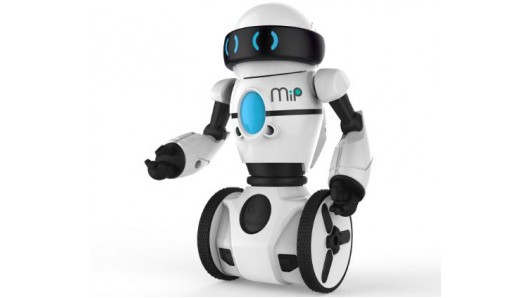
\includegraphics[width=\linewidth]{figures/robot.jpg}
\end{minipage}
\end{figure}
\vspace{1cm}
\thispagestyle{empty}
\begin{abstract}
This report describes the work done for the Robotics and Autonomous Systems project. The task consisted on designing a robot that would be able to autonomously explore a maze, avoid obstacles, detected and identify objects and build a map as it navigates. In addition, on a second run, it had to be able to "fetch" the objects as fast as possible using the previously acquired knowledge. The robot was tested in the laboratory and in a contest with satisfactory results. Finally, a performance analysis and some conclusions summarize this report. 
\end{abstract}
\end{titlepage}

%===============================================================================
\begingroup
\hypersetup{linkcolor=black}
\tableofcontents
\endgroup
\newpage
%===============================================================================

\section{Introduction\label{sec:Introduction}}
This report describes the work done for the final project for the course Robotics and Autonomous systems. The purpose is to reflect about ideas and solutions we provided in order to try to reach the goal of this course – making autonomous robot that can explore maze, create map of it and detect and recognize different geometrical objects located in maze.


%===============================================================================

\section{Mechanical design \label{sec:Mechanics}}
The robot was built following a standard differential drive configuration (XXXX reference) because of an easier control (e.g.: rotate around it's center point without moving). A picture of the robot can be seen in Figure \ref{fig:robotPic}.

\begin{figure}[h]
        \centering
        \begin{subfigure}[b]{0.45\linewidth}
        \centering
                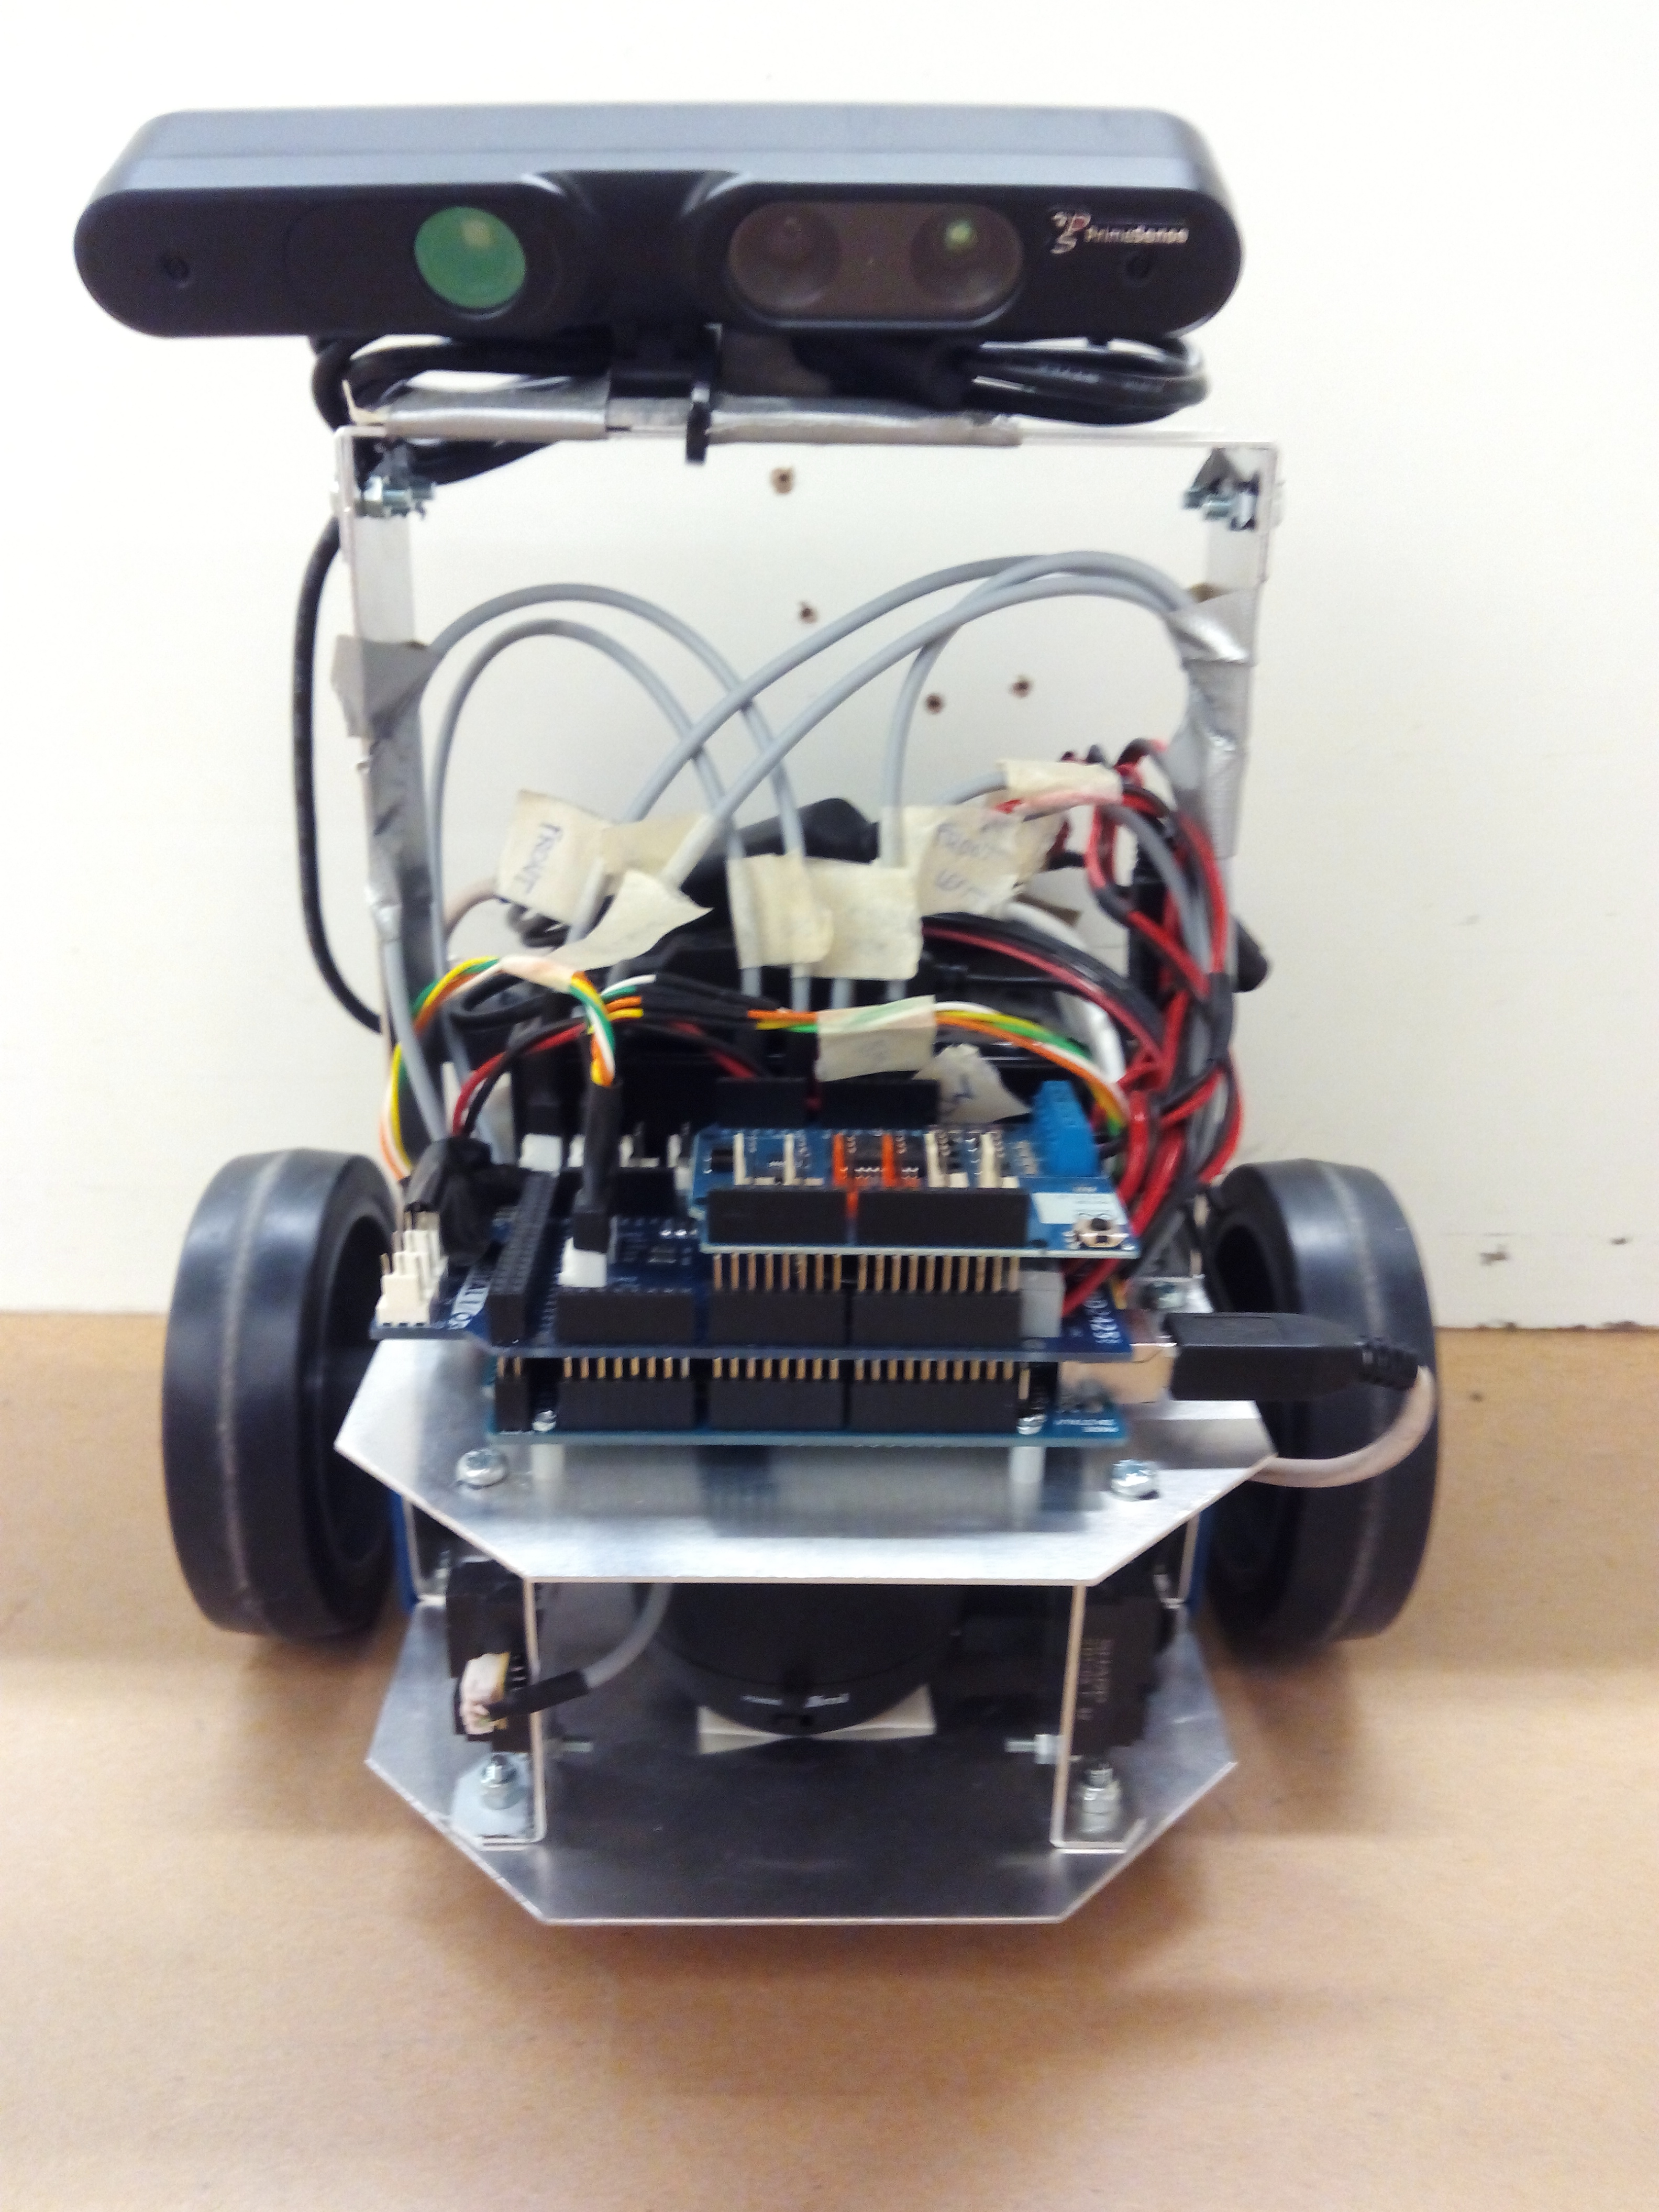
\includegraphics[height=5cm]{figures/front.jpg}
		\caption{Front view}
        \end{subfigure}
        \begin{subfigure}[b]{0.45\linewidth}
        \centering
                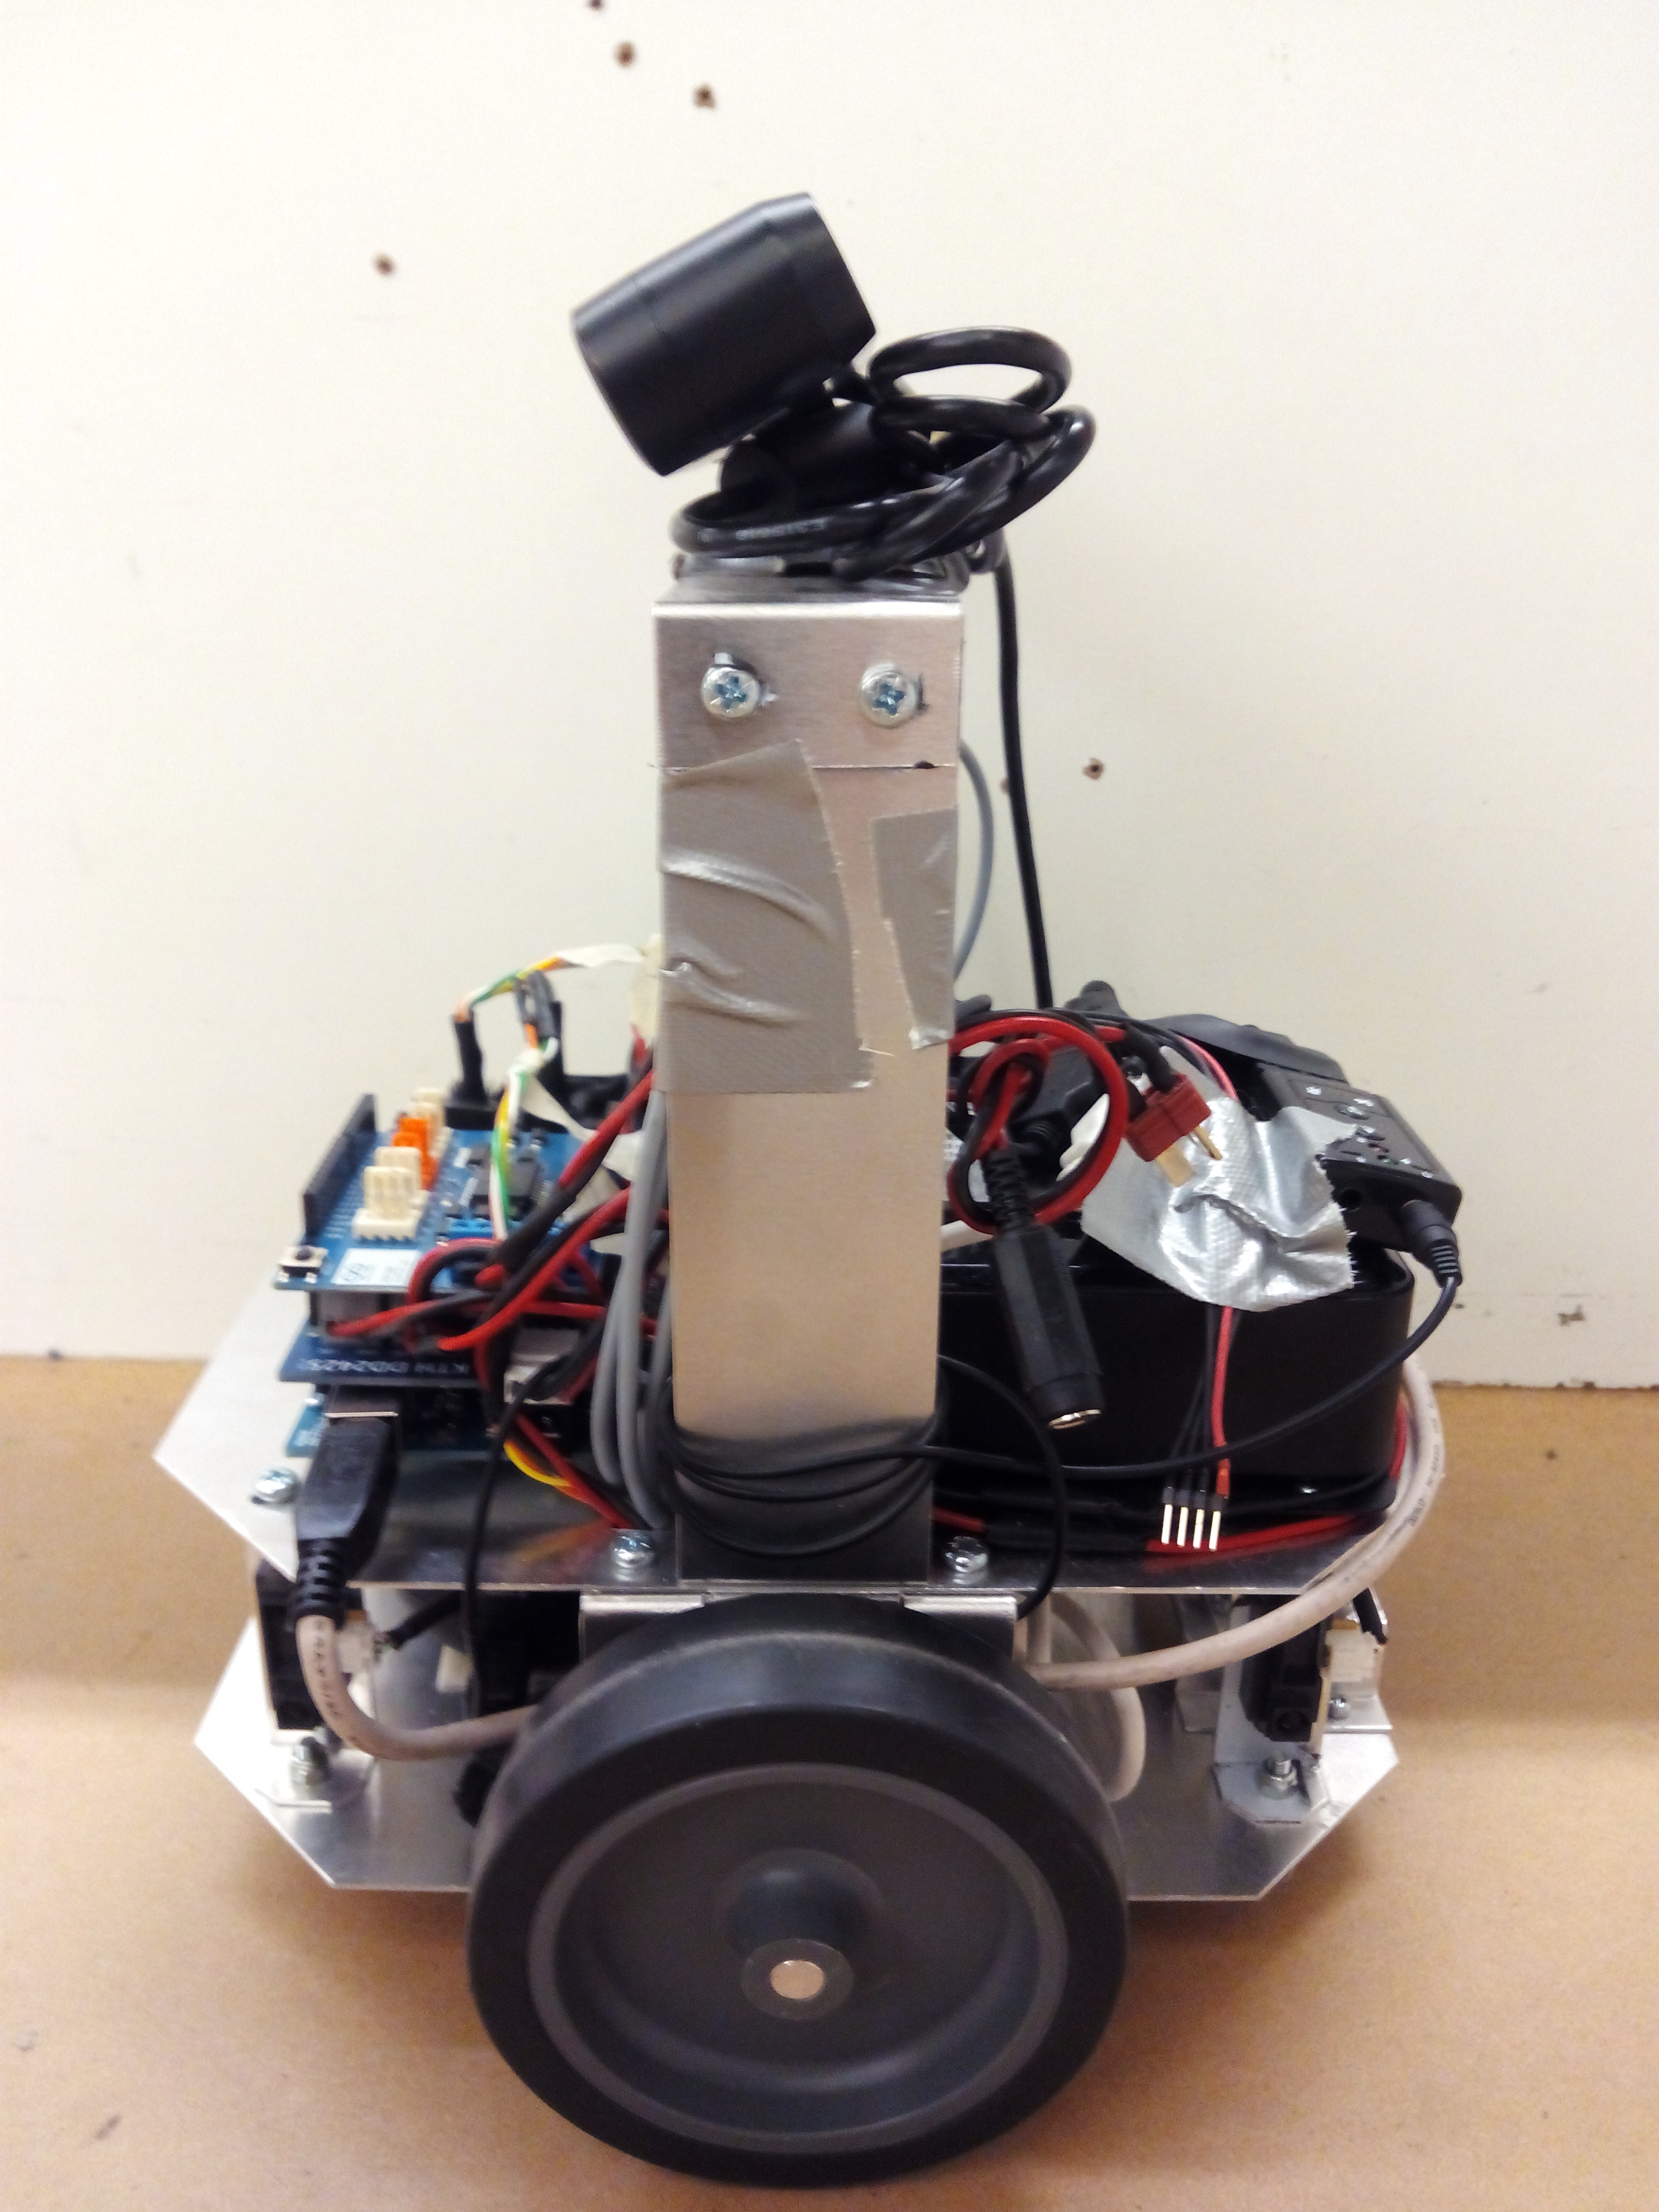
\includegraphics[height=5cm]{figures/side.jpg}
                \caption{Side view}
        \end{subfigure}
        \caption{Pictures of the robot}
                \label{fig:robotPic}
\end{figure}


The dimensions are 23 cm x 23 cm wide and long (including wheels) and 29 cm high. Two aluminium plates are connected with four pillars in order to create two floors. On the first floor are located motors, the battery and speaker whereas on the second floor the NUC and the Arduino sandwich can be found. For camera there is pillar which raises it high enough so it reaches 29 cm height. This is required in order to get depth information, which requires a minimum distance of 35 cm from the camera. The IMU is located at the center of the robot, under the second plate, as well as the long range IR sensors looking forward and backwards. The short range IR sensors are located on the pillars which connect first and second floor, with the aim of performing wall following. 

%===============================================================================

\section{Electronics}
The robot includes the following components:
\begin{itemize}
\item Intel NUC computer.
\item Arduino Mega 2560 + Motor Shield + custom I/O board.
\item PrimeSense RGB-D 1.09 sensor.
\item 2 motors + wheels
\item 4 Sharp GP2D120 (short range)
\item 2 Sharp GP2D12 (long range)
\item IMU Phidgets
\item Speaker + sound card
\item LiPo battery 3-cell 5000 mAh.
\end{itemize}

\subsection{IR sensors}
\subsubsection{Calibration}

Because of non-linear sensor output vs distance curve it is not practical to use raw values from IR sensors in higher level nodes. Therefore it was needed to create node which converts raw data from sensors to distance. As the raw output changes values more rapidly in lower distances, measurements in low range were made quite densely (by measuring sensor output every 0.5 cm) whereas in longer distances such accuracy were not needed because output values were approximately the same even within 5 cm range. Sensor converter node is the only one which subscribes to raw sensors node and other nodes in ROS subscribes directly to distance data.

\subsubsection{Filtering}

To filter out the noise from the IR sensors a set of independent Kalman Filters \cite{Thrun} is used due to its simplicity and ability to directly model the sensor and process noise. 
In particular, we consider the following process and measurement models:
\begin{align*}
x_{t+1} &= x_t + \epsilon \\
z_t &= x_t + \delta
\end{align*}
, where $\epsilon \sim \mathcal{N}(0,Q)$ and $\delta \sim \mathcal{N}(0,R)$. A value of $R = 0.01$, $Q = 0.04$ was chosen in order to effectively filter but not reduce the bandwidth (responsiveness) too much. 

%===============================================================================

\section{Motion control}
To be able to reliably use motors instead of sending just PWM data to motors there needs to be a node which translates linear and angular speeds to necessary PWM values. However as PWM vs speed relation is highly non-linear and depends on many factors such as ground friction it is not possible to just find suitable function for translating speed to PWM. The use of motor controller is therefore crucial. Its task is to control PWM values at the same time getting feedback from encoders. This data then can be used to adjust PWM values so that motor reaches the necessary speed and keeps it. In this project PID controller is used for motor control. Equation \ref{eq:pid_equation} shows general PID controller algorithm. In case of motor controller error e(t) is difference between desired angular speed and current angular speed which can be calculated with equation \ref{eq:pid_error}. N describes ticks per revolution.

\begin{align}
\label{eq:pid_equation}
u(t) = K_p e(t) + K_i \int_{0}^{t} e(\tau) d\tau + K_d \frac{de(t)}{dt} 
\end{align}
\begin{align}
\label{eq:pid_error}
\omega (t) = \frac{2 \pi \Delta encoder}{\Delta t * N}
\end{align}

With PID controller it is very important to find right parameters otherwise motion can be with oscillations, too slowly rising or could have other problems. 

XXXX Translation between v and w to wwheel

Distinguish low-level and high-level control

Non-linearity in motors

%===============================================================================

\section{Software}
In this project ROS software is used. It creates good and feature rich environment for simple nodes which can easily communicate to each other.

\subsection{Global picture}
\subsection{Odometry}

Odometry node takes raw data from motor encoders and translates it into global coordinates and angle according to equations \ref{eq:odometry_eq}. This data can be used for mapping and localization. Problem with odometry is that it tends to drift especially when speed increases.

\label{eq:odometry_eq}
\begin{align}
distance _{left} = \frac{2\pi * Wheel radius * encoder _{left}}{ticks  per  revolution}  \\
distance _{right} = \frac{2\pi * Wheel radius * encoder _{right}}{ticks  per  revolution} \\
\Delta x = \frac{distance _{left} + distance _{right}}{2} * cos(\Phi) \\
\Delta y = \frac{distance _{left} + distance _{right}}{2} * sin(\Phi) \\
\Delta \Phi = \frac{distance _{left} - distance _{right}}{Wheelbase}
\end{align}




\subsection{Mapping}

For map we chose to use occupancy grid package from ROS. IR sensors provide data about distances to the walls. This data together with position information from odometry node are used to make a map. Initially all area is unknown and by driving around and getting corresponding data from IR sensors free area and obstacles are detected and drawn in map. Data from sensors are quite noisy therefore some processing is needed to mitigate noisy results.

\subsection{Exploration}

For exploration there was created navigation node. 

\subsubsection{Wall following}
\subsubsection{BFS Search}
\subsection{Path planning}
\subsubsection{Local}

\subsubsection{Global}
The global path planning consists on determining the fastest sequence of objects to be visited. This is applied in Phase 2 during the contest. 

This is a classical formulation of the Travelling Salesman Problem (TSP). XXXXX ref Here objects can be considered as nodes within a graph and edges that connect them with some cost.

In our particular case, we propose the following formulation:
\begin{itemize}
\item The nodes are \textbf{not} the object's position, but the position from which the robot first saw the object instead. This is done to make the path planning easier: since the objects are commonly really close to walls, we might not even find a path to them considering that it is computed is the "thickened" map. 
\item The cost between two objects is measured in terms of the \textbf{travel distance}, measured as the size of the path computed from running a Best-First Search from one object to another. This metric is much better than just using the Euclidean Distance between objects (for example, consider the case where the objects are separated by just a wall but the robot cannot go through that wall and has to turn around instead). Even a more accurate metric would include an additional cost for turning, but we did not include this in our formulation.
\end{itemize}

Therefore, after Phase 1 we can create a high-level graph connecting all the object's positions with the associated costs. 

\textbf{Solution: Genetic Algorithm}\\
Once the TSP problem, we find the best solution for it. As XXXXX shows, this is an NP-hard problem, which means it cannot be solved in polynomial time with standard search algorithms. Instead, a very elegant solution is to use a Genetic Algorithm (GA) XXXX ref, which we apply to this particular problem. The main advantages for this is that it is simple to implement and understand, really scalable and offers a good trade-off between computational time and optimality. 

The mechanism behind the GA is quite common and the reader is referred to XXXX to get more details about it. We will mention here the relevant details:
\begin{itemize}
\item \textbf{Codification}. Genetic algorithms work with strings of chromosomes, so we need to somehow encode the graph information into a string. For this, we gave an integer ID number to each of the nodes, and formed a string as a sequence of IDs (see Figure XXXX).
\item \textbf{Fitness function}. It determines the performance of a single individual from a generation. We choose the fitness of individual $i$ to be:
\begin{align}
f(i) = \left[\sum_{i = 1}^{N-1} C(i,i+1)\right]^{-1}
\end{align}
, where $C(i, i+1)$ is the travel cost of going from node $i$ to node $i+1$, and $N$ is the total number of nodes.
\item Parameters. 
\begin{itemize}
\item Number of generations: 2000.
\item Number of individuals per generation: 100
\item Number of ellite individuals: 2
\item Cross-over probability: 0.7
\item Mutation probability: 0.05
\end{itemize}
\end{itemize}

This implementation gave excellent results, with nearly optimal solutions under a reduced time (around 1.0 s on the NUC). Figure XXXX shows an example test with a graph with 20 nodes. 



\subsection{Localization}
Given the lack of time for the project, it was not possible to achieve a fully working localization module, which was really an impediment for running Phase 2. The following solutions were tested.

\subsubsection{EKF Localization}
Following the theory from the Applied Estimation course (XXX REF), we found out that a good solution was to use an Extended Kalman Filter (XXXX REF) to solve this problem. It would use as input $u$ the data from the encoders, and the measurements would come from a \emph{range-and-bearing} sensor, which provides the distance and angle to a recognized object in the map relative to the robot, as shown in Figure XXXX.

The implementation followed the instructions in XXXXX REF, but the results were not so good. A really large process noise ($Q$) and really low measurement noise ($R$) was required to notice some updated in the position. However, we discarded this idea when we realized that the localization could be non-unique: the same $\theta$ and $\rho$ could be obtained at any position on a circle of radius $\rho$ around the object, given a proper orientation for the robot. In addition, the object's position would not be stable enough to heavily rely on this information. 

\subsubsection{Theta correction}
A solution which did work was to compute the actual orientation of the robot from it's orientation with respect to the wall. This can be shown in Figure XXXXX


From this, the difference in angle, $\Delta\theta$, can be computed as:
\begin{align}
\label{eq:locTheta}
\Delta\theta = \tan^{-1}\left(\frac{d_2 - d_1}{D}\right)
\end{align}

Finally, we assume the robot has an orientation $\theta0 \in \{-\pi, -\pi/2, 0, \pi/2, \pi\}$, so the final pose estimate is given by: $\theta = \theta0 + \Delta\theta$.

This was applied when starting the robot and it worked pretty well; however this could not be applied afterwards since wall following or 90-degree turning were not used in the end in favour of just path following.  

\subsubsection{On-line localization}
Finally, we implemented a promising idea for localization, but we did not have the time to test and debug it properly. The algorithm is as follows:

\begin{itemize}
\item The current pose estimate ${x_0, y_0, theta_0}$ and a map (occupancy grid) are given.

\item The orientation ($\theta$) is updated according to the previous section.

\item We define a search region around the current pose estimate in X and Y coordinates (e.g.: a square of $10\times10$ cm.
\item Every position $\{x,y\}$ inside that region (within some discretization margin) is assigned a cost based the current sensor readings and the map, according to Equation \ref{eq:localization}.
\begin{align}
\label{eq:localization}
J(x,y) = \sum_{i = 1}^6 (z_i - \hat{z}_i)
\end{align}
, where $z_i$ is the current sensor reading for the $i$th sensor reading, and $\hat{z}_i$ is the \emph{expected} sensor reading from the position $\{x,y\}$. This is done by raycasting from every sensor position to the saved map.

\item The new position is updated as follows:
\begin{align}
\{x,y\} = \arg\max_{x,y}J(x,y)
\end{align}

\end{itemize}


This approach would give the optimal robot position assuming that the saved map was perfect and we were given perfect sensor readings. Unfortunately this was not the case. In addition, another challenging question is when to run this procedure. Ideally, it would be better to run it after 90-degree turns, but again that was not used in the robot anymore. We are confident that a little bit more time to improve this and test would have probably resulted in satisfactory results.

%===============================================================================

\section{Computer Vision}
\subsection{Camera extrinsic calibration}
\subsection{Object detection}
\subsection{Object recognition}
\subsection{Obstacle detection}


%===============================================================================

\section{Discussion}
\subsection{Results}
\subsection{System Evaluation}
\subsection{Project management}

%===============================================================================

\section{Conclusions}
Conclusions

%===============================================================================
\begin{appendices}
\section{Schematics}
The contents...
\end{appendices}


\newpage
\printbibliography 

\end{document}